%---------------------------------------------------------------------
%
%                          Ap�ndice A
%
%---------------------------------------------------------------------
\chapter{Traducci�n de los corpus mediante Text2LSE}.
\label{ap1:F}
%-------------------------------------------------------------------
\section{Corpus de oraciones de instrucciones de seguridad de un vuelo}
%-------------------------------------------------------------------
\begin{enumerate}
  \item Hola, les damos la bienvenida a este vuelo de Iberia en nuestro nombre y en el de Madrid. 
 \begin{figure}[H]
 	\centering
 	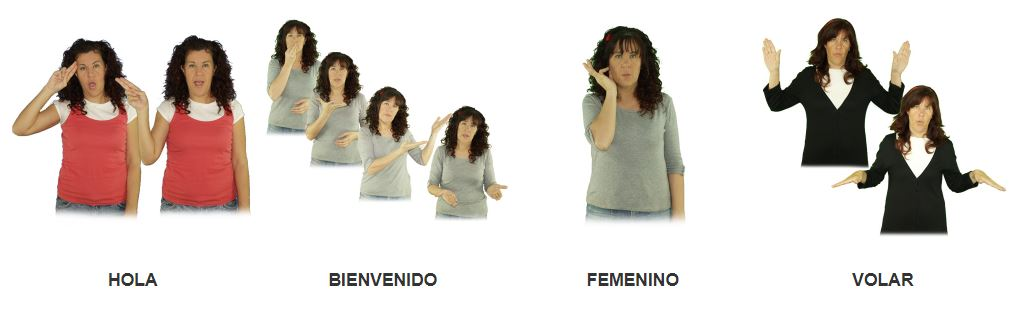
\includegraphics[width=0.9\textwidth]{Imagenes/Fuentes/apendices/A1_1.jpg}
 	\label {fig: AP_A1.1}
 \end{figure}
\begin{figure}[H]
	\centering
	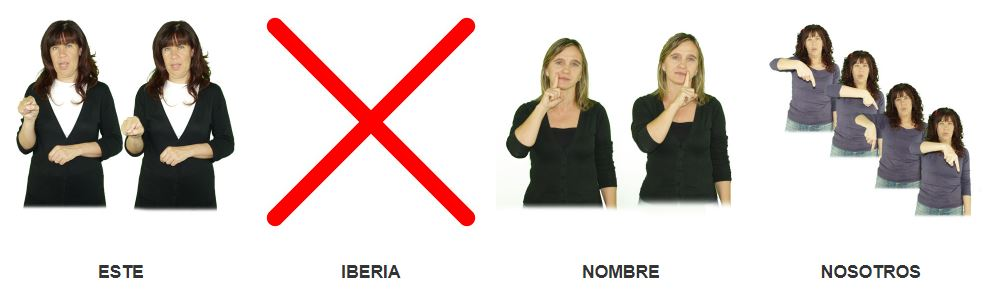
\includegraphics[width=0.9\textwidth]{Imagenes/Fuentes/apendices/A1_2.jpg}
	\label {fig: AP_A1.2}
\end{figure}
\begin{figure}[H]
	\centering
	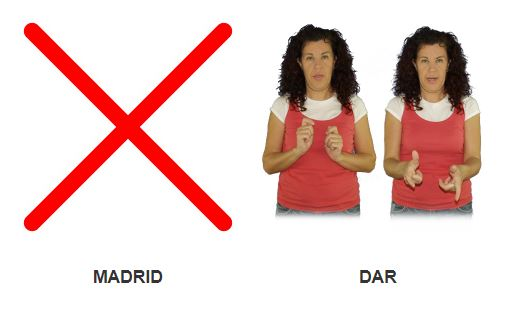
\includegraphics[width=0.9\textwidth]{Imagenes/Fuentes/apendices/A1_3.jpg}
	\label {fig: AP_A1.3}
\end{figure}
 
 \item Antes de despegar tenemos que darles unas instrucciones de seguridad. 
 
 \begin{figure}[H]
 	\centering
 	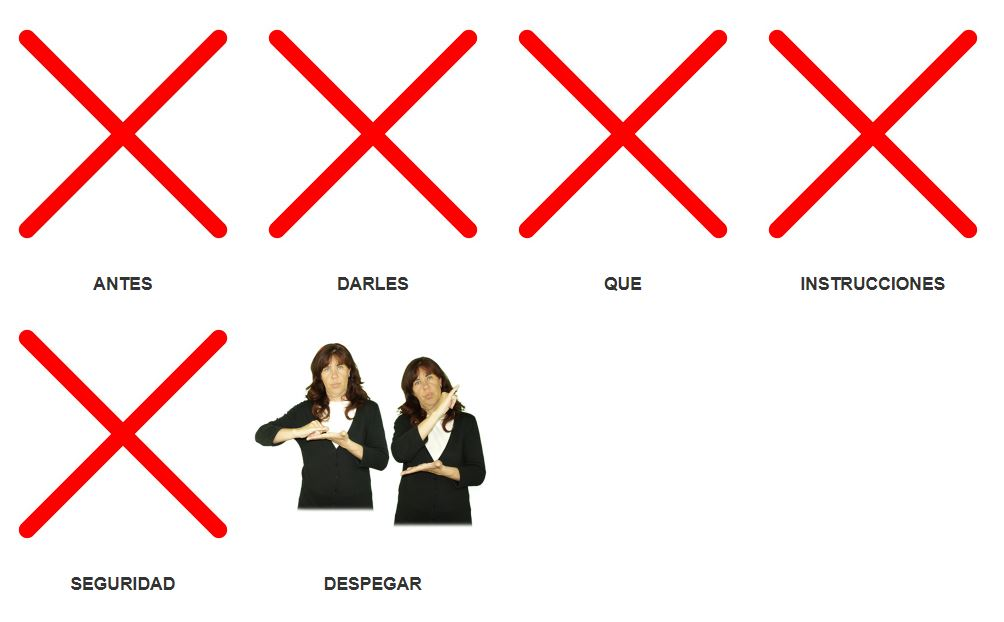
\includegraphics[width=0.9\textwidth]{Imagenes/Fuentes/apendices/A2.jpg}
 	\label {fig: AP_A2}
 \end{figure}
 
 \item Es importante que presten atenci�n. 
 
 \begin{figure}[H]
 	\centering
 	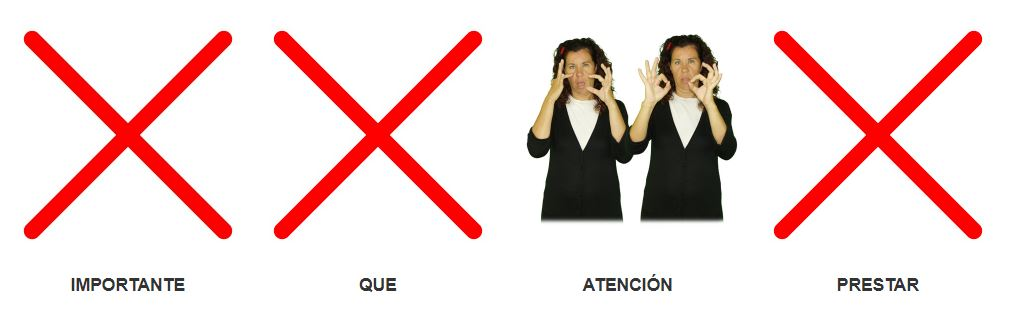
\includegraphics[width=0.9\textwidth]{Imagenes/Fuentes/apendices/A3.jpg}
 	\label {fig: AP_A3}
 \end{figure}
 
 \item Durante el despegue y aterrizaje. 
 
 \begin{figure}[H]
 	\centering
 	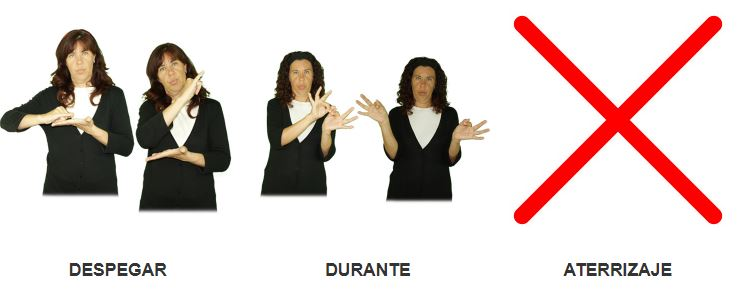
\includegraphics[width=0.9\textwidth]{Imagenes/Fuentes/apendices/A4.jpg}
 	\label {fig: AP_A4}
 \end{figure}
 
 \item Los dispositivos electr�nicos deber�n permanecer desenchufados y en modo avi�n. 
 
 \begin{figure}[H]
 	\centering
 	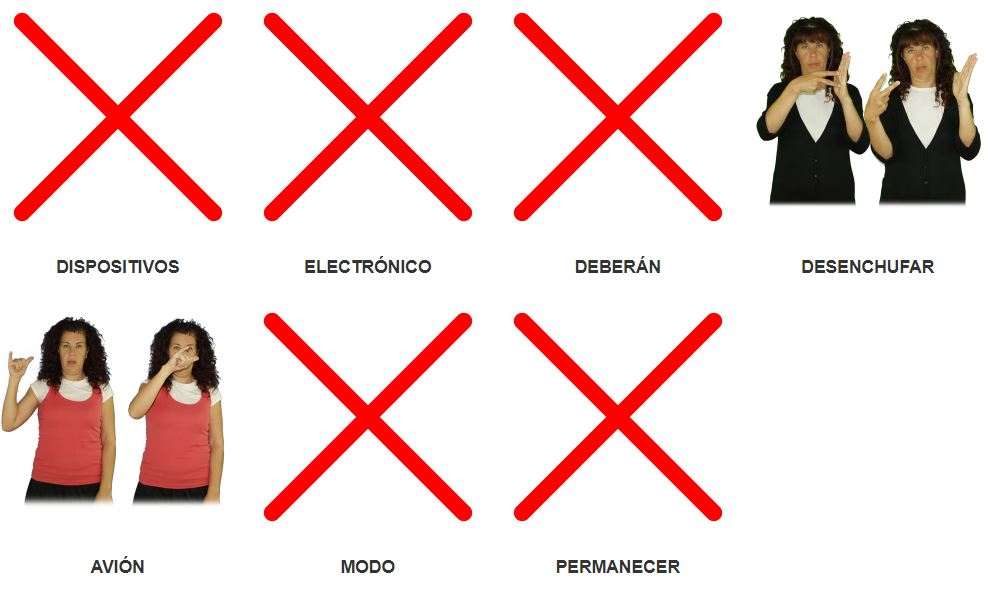
\includegraphics[width=0.9\textwidth]{Imagenes/Fuentes/apendices/A5.jpg}
 	\label {fig: AP_A5}
 \end{figure}
 
 \item Despu�s podr�n utilizarlos durante todo el vuelo.
 
 \begin{figure}[H]
 	\centering
 	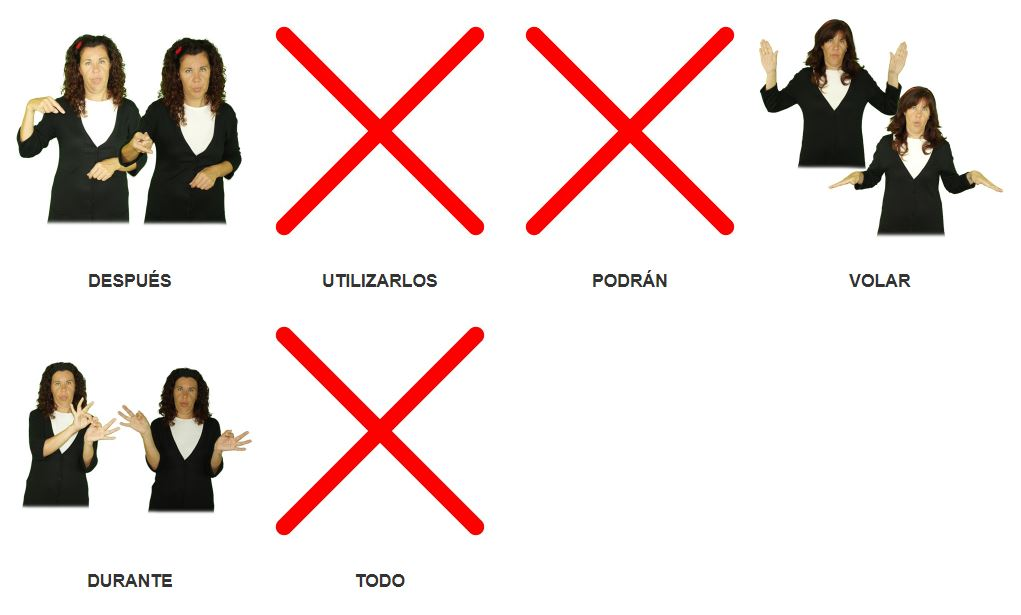
\includegraphics[width=0.9\textwidth]{Imagenes/Fuentes/apendices/A6.jpg}
 	\label {fig: AP_A6}
 \end{figure}
 
 \item Excepto cuando la tripulaci�n les pida que los apaguen. 
 
 \begin{figure}[H]
 	\centering
 	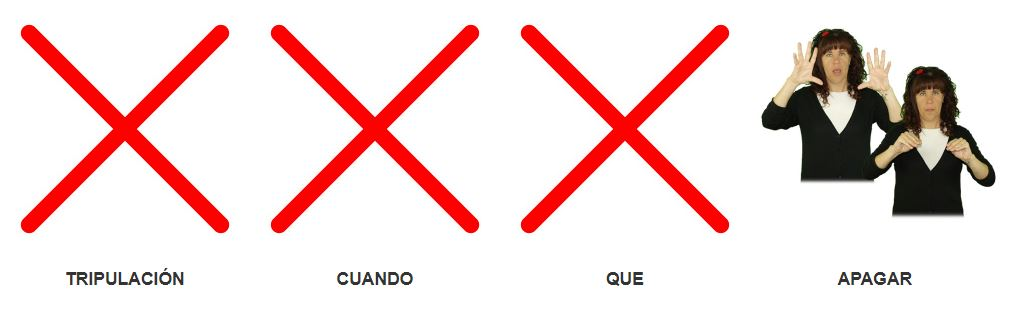
\includegraphics[width=0.9\textwidth]{Imagenes/Fuentes/apendices/A7.jpg}
 	\label {fig: AP_A7}
 \end{figure}
 
 \item Recuerden que este avi�n dispone de conexi�n Wifi.
 
 \begin{figure}[H]
 	\centering
 	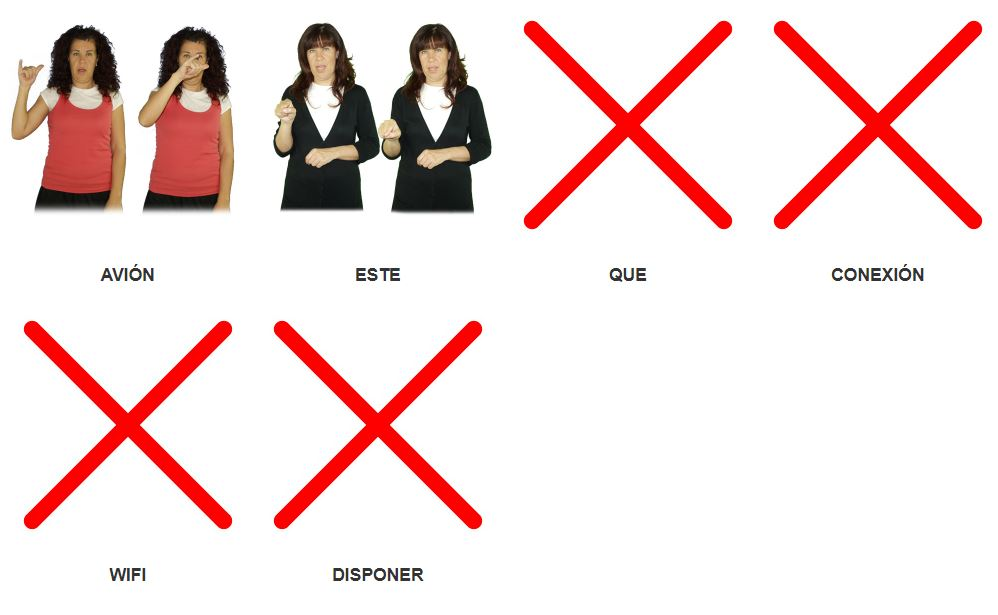
\includegraphics[width=0.9\textwidth]{Imagenes/Fuentes/apendices/A8.jpg}
 	\label {fig: AP_A8}
 \end{figure}

 \item Y que podr�n conectarse a Internet cuando se lo comuniquemos. 
 
 \begin{figure}[H]
 	\centering
 	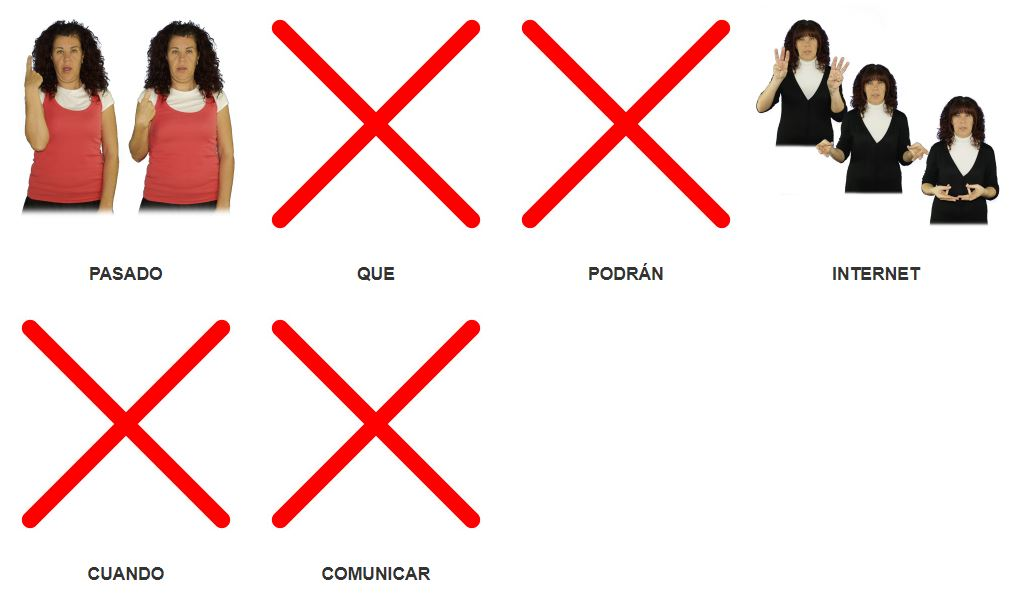
\includegraphics[width=0.9\textwidth]{Imagenes/Fuentes/apendices/A9.jpg}
 	\label {fig: AP_A9}
 \end{figure}
 
 \item Si han tra�do equipaje de mano.
 
  \begin{figure}[H]
 	\centering
 	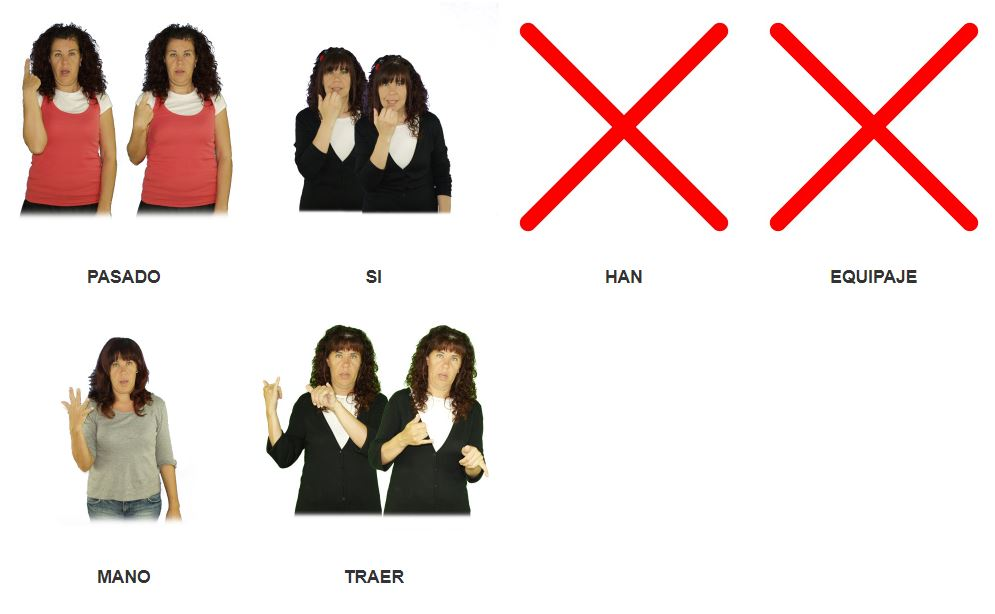
\includegraphics[width=0.9\textwidth]{Imagenes/Fuentes/apendices/A10.jpg}
 	\label {fig: AP_A10}
 \end{figure}
 
 \item Por favor, col�quelo en los compartimentos situados encima de sus butacas o debajo de sus asientos delanteros.
 
  \begin{figure}[H]
 	\centering
 	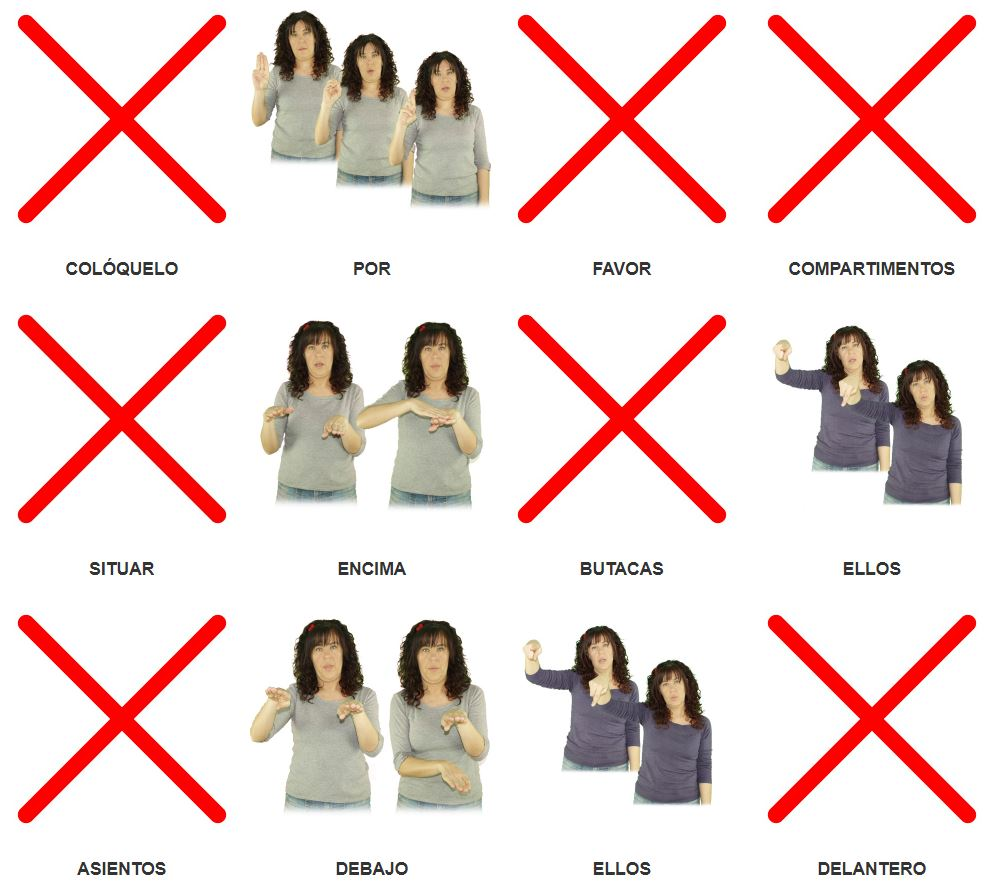
\includegraphics[width=0.9\textwidth]{Imagenes/Fuentes/apendices/A11.jpg}
 	\label {fig: AP_A11}
 \end{figure}
 
 \item Dejando despejados los pasillos y salidas de emergencia. 
 
   \begin{figure}[H]
 	\centering
 	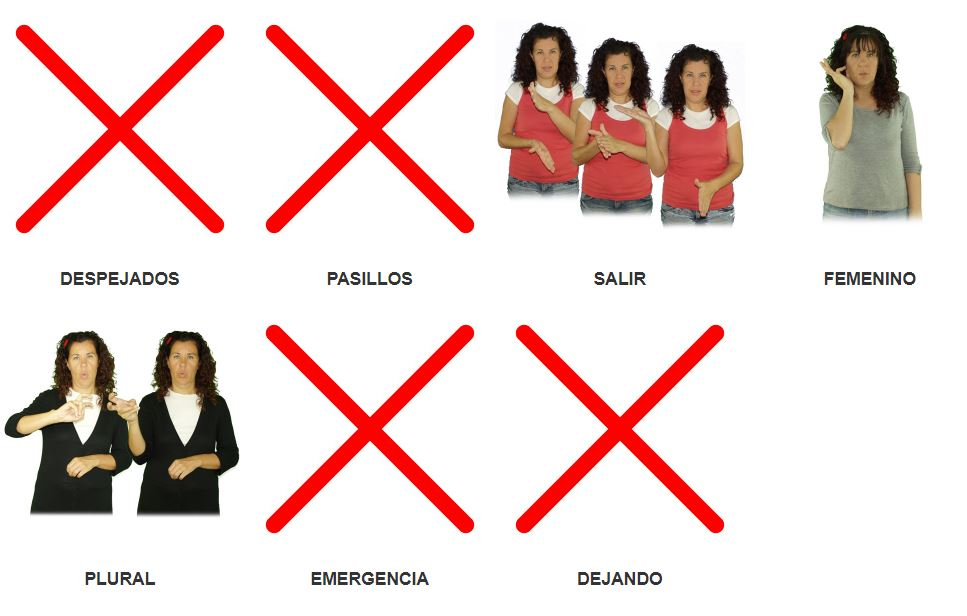
\includegraphics[width=0.9\textwidth]{Imagenes/Fuentes/apendices/A12.jpg}
 	\label {fig: AP_A12}
 \end{figure}
 
 \item Durante el vuelo podr�n ponerse c�modos.
 
\begin{figure}[H]
 	\centering
 	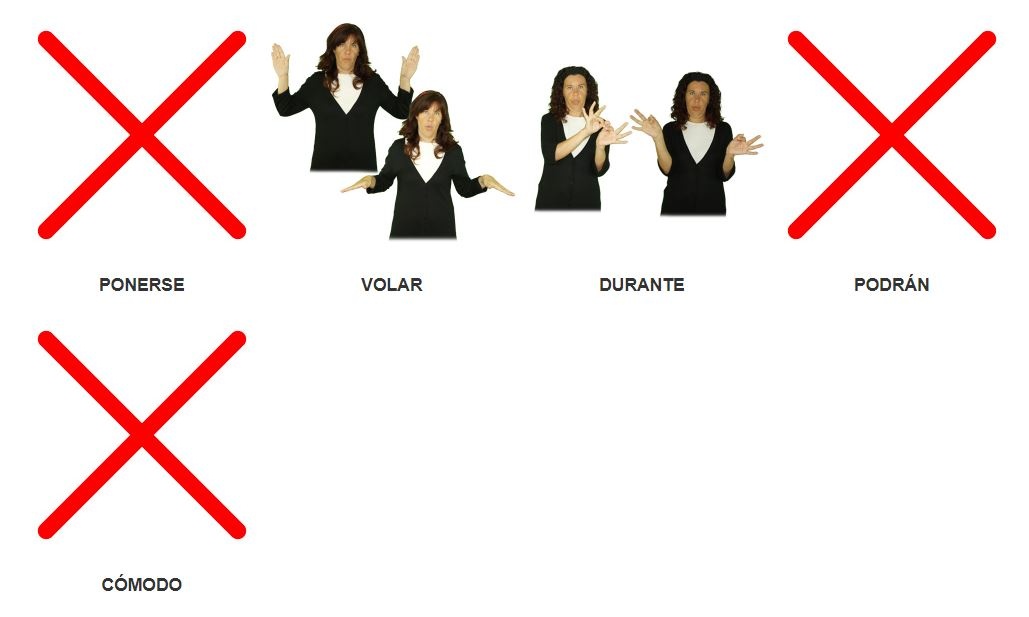
\includegraphics[width=0.9\textwidth]{Imagenes/Fuentes/apendices/A13.jpg}
 	\label {fig: AP_A13}
 \end{figure}
 
 \item Pero durante el despegue y aterrizaje.
 
 \begin{figure}[H]
 	\centering
 	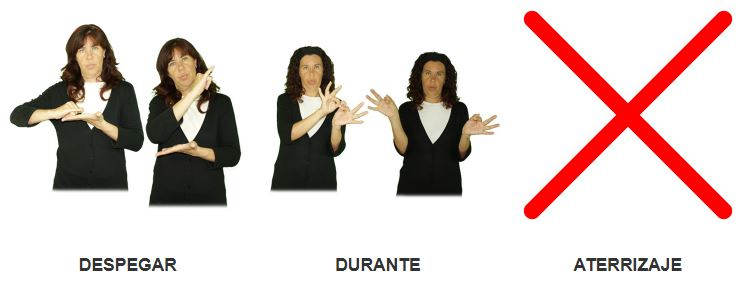
\includegraphics[width=0.9\textwidth]{Imagenes/Fuentes/apendices/A14.jpg}
 	\label {fig: AP_A14}
 \end{figure}
 
 \item Por favor, pongan sus asientos en posici�n vertical.
 
  \begin{figure}[H]
 	\centering
 	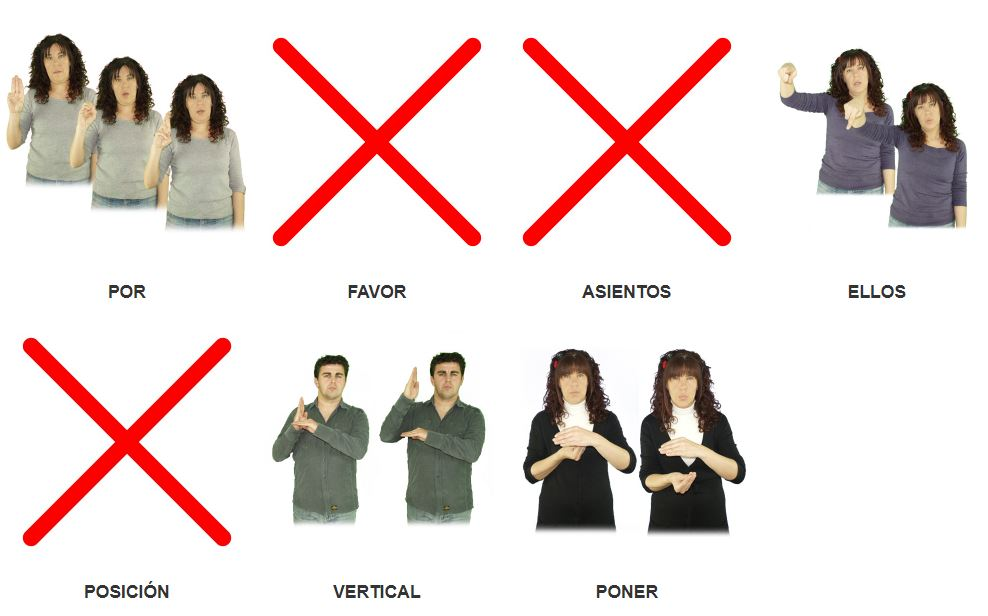
\includegraphics[width=0.9\textwidth]{Imagenes/Fuentes/apendices/A15.jpg}
 	\label {fig: AP_A15}
 \end{figure}
 
 \item Y mantengan su mesa plegada. 
 \item Por su seguridad.
 \item Les recomendamos que mantengan su cintur�n abrochado y visible durante todo el vuelo. 
 \item Y siempre que la se�al luminosa lo indique. 
 \item Para abrocharlo.
 \item Inserte la trabilla en su enganche correspondiente. 
 \item Para soltarlo.
 \item Simplemente levanten la leng�eta del enganche. 
 \item Este avi�n cuenta con ocho puertas y dos ventanas de salida, 4 puertas a cada lado del avi�n y una ventana sobre cada ala. 
 \item Todas est�n se�alizadas con la palabra EXIT. 
 \item Y disponen de rampas o balsas de evacuaci�n. 
 \item Debajo de sus asientos encontrar�n un chaleco salvavidas. 
 \item S�quenlo de la bolsa.
 \item Y para pon�rselo.
 \item Introduzcan la cabeza por la abertura.
 \item Y pasen la cinta de atado por detr�s de su cintura.
 \item Enganchando la fijaci�n de la hebilla de un extremo a otro. 
 \item Y tirando de la cinta para ajust�rselo. 
 \item Para inflarlo.
 \item Solo tienen que tirar con fuerza del tirador del pl�stico rojo.
 \item O soplar por el tubo. 
 \item Y recuerden.
 \item Nunca deben inflar el chaleco dentro del avi�n. 
 \item En caso de despresurizaci�n de la cabina.
 \item Se abrir� autom�ticamente un compartimento sobre sus asientos.
 \item Que contiene m�scaras de ox�geno. 
 \item Tire de la suya.
 \item Col�quela sobre su nariz y boca.
 \item Y respire con normalidad. 
 \item Despu�s preste ayuda a qui�n pueda depender de usted. 
 \item Recuerden.
 \item Que para evitar poner en peligro la seguridad de este vuelo.
 \item No est� permitido fumar.
 \item O usar dispositivos de liberaci�n de nicotina en ning�n caso. 
 \item Y no olviden.
 \item Que tienen m�s informaci�n en las instrucciones de seguridad.
 \item Que encontrar�n en la bolsa delantera de sus asientos. 
 \item Muchas gracias por su atenci�n. 
 \item Esperamos que disfruten de un feliz vuelo.
 
\end{enumerate}


  